\noindent
\subsection{Author based features}
\label{author_analysis}

We next look into some of the author based features like author reputation and author productivity to determine how they influence the long-term citation of the paper.  
\begin{figure*}
\centering
\begin{tabular}{ccc}
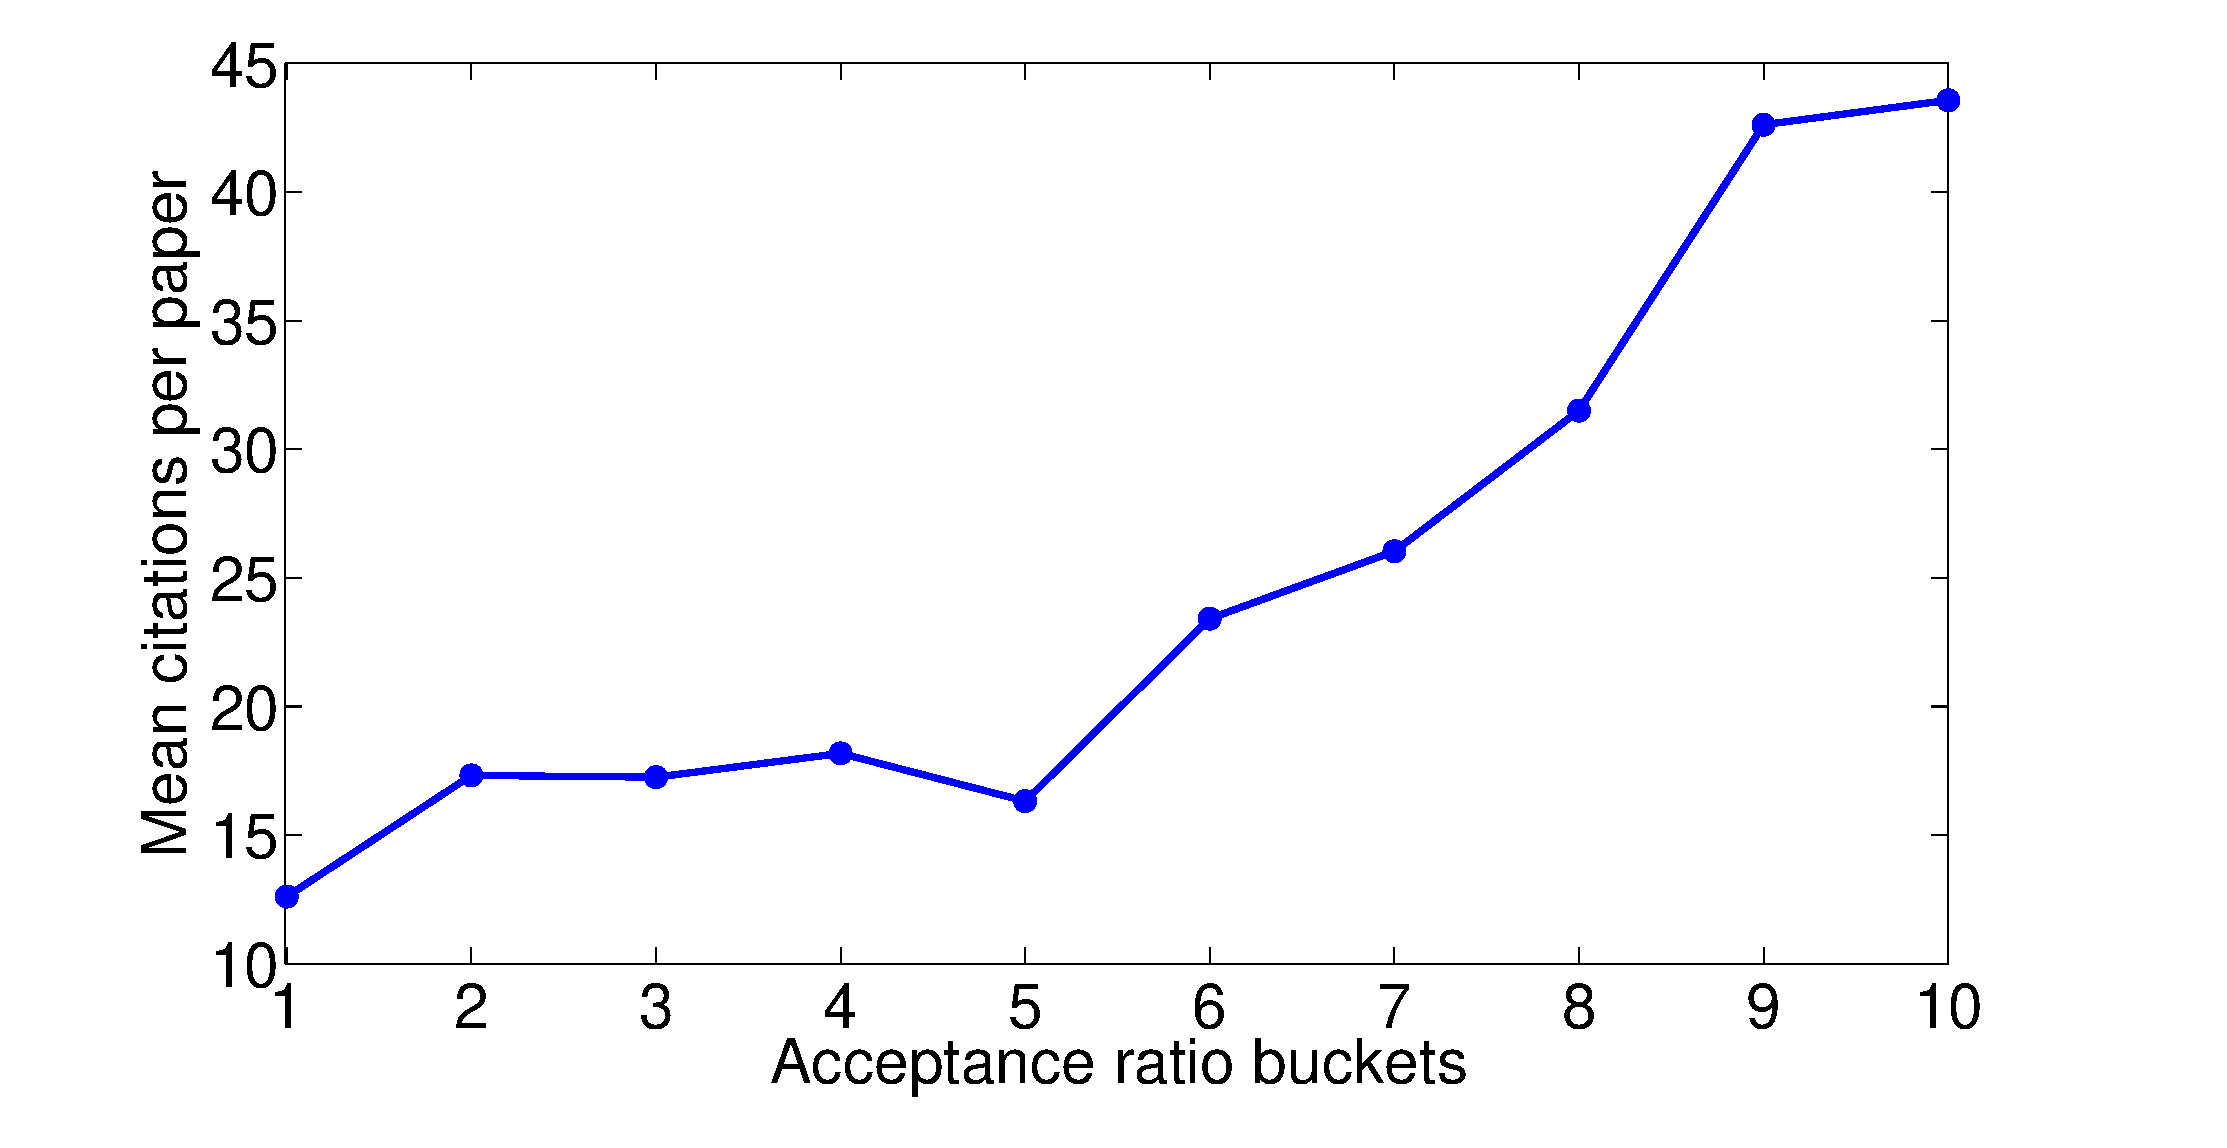
\includegraphics[scale=0.15]{figures/citation_succes_ratio.eps} & 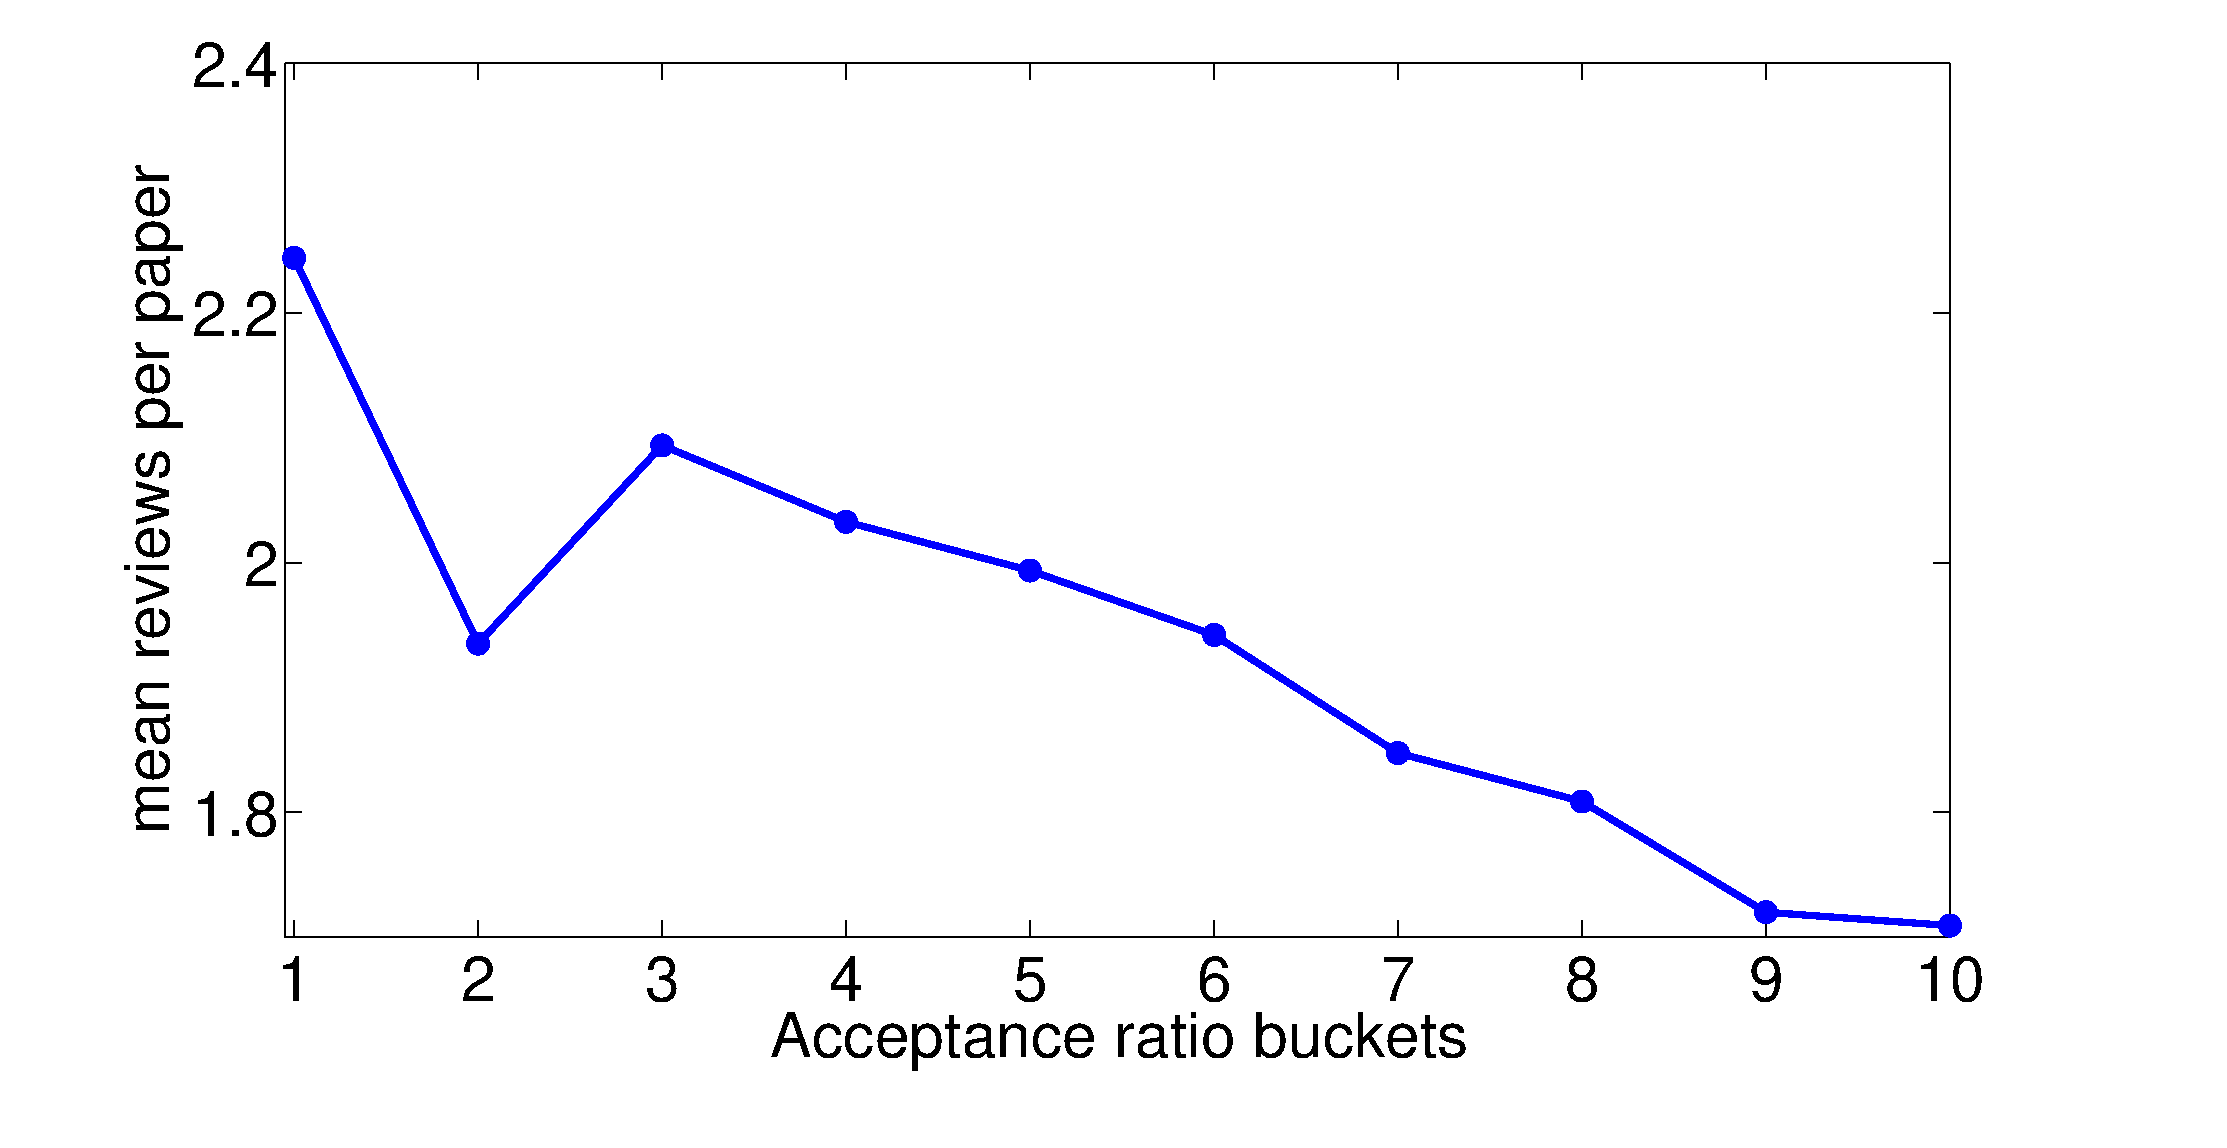
\includegraphics[scale=0.15]{figures/review_succes_ratio.eps} & 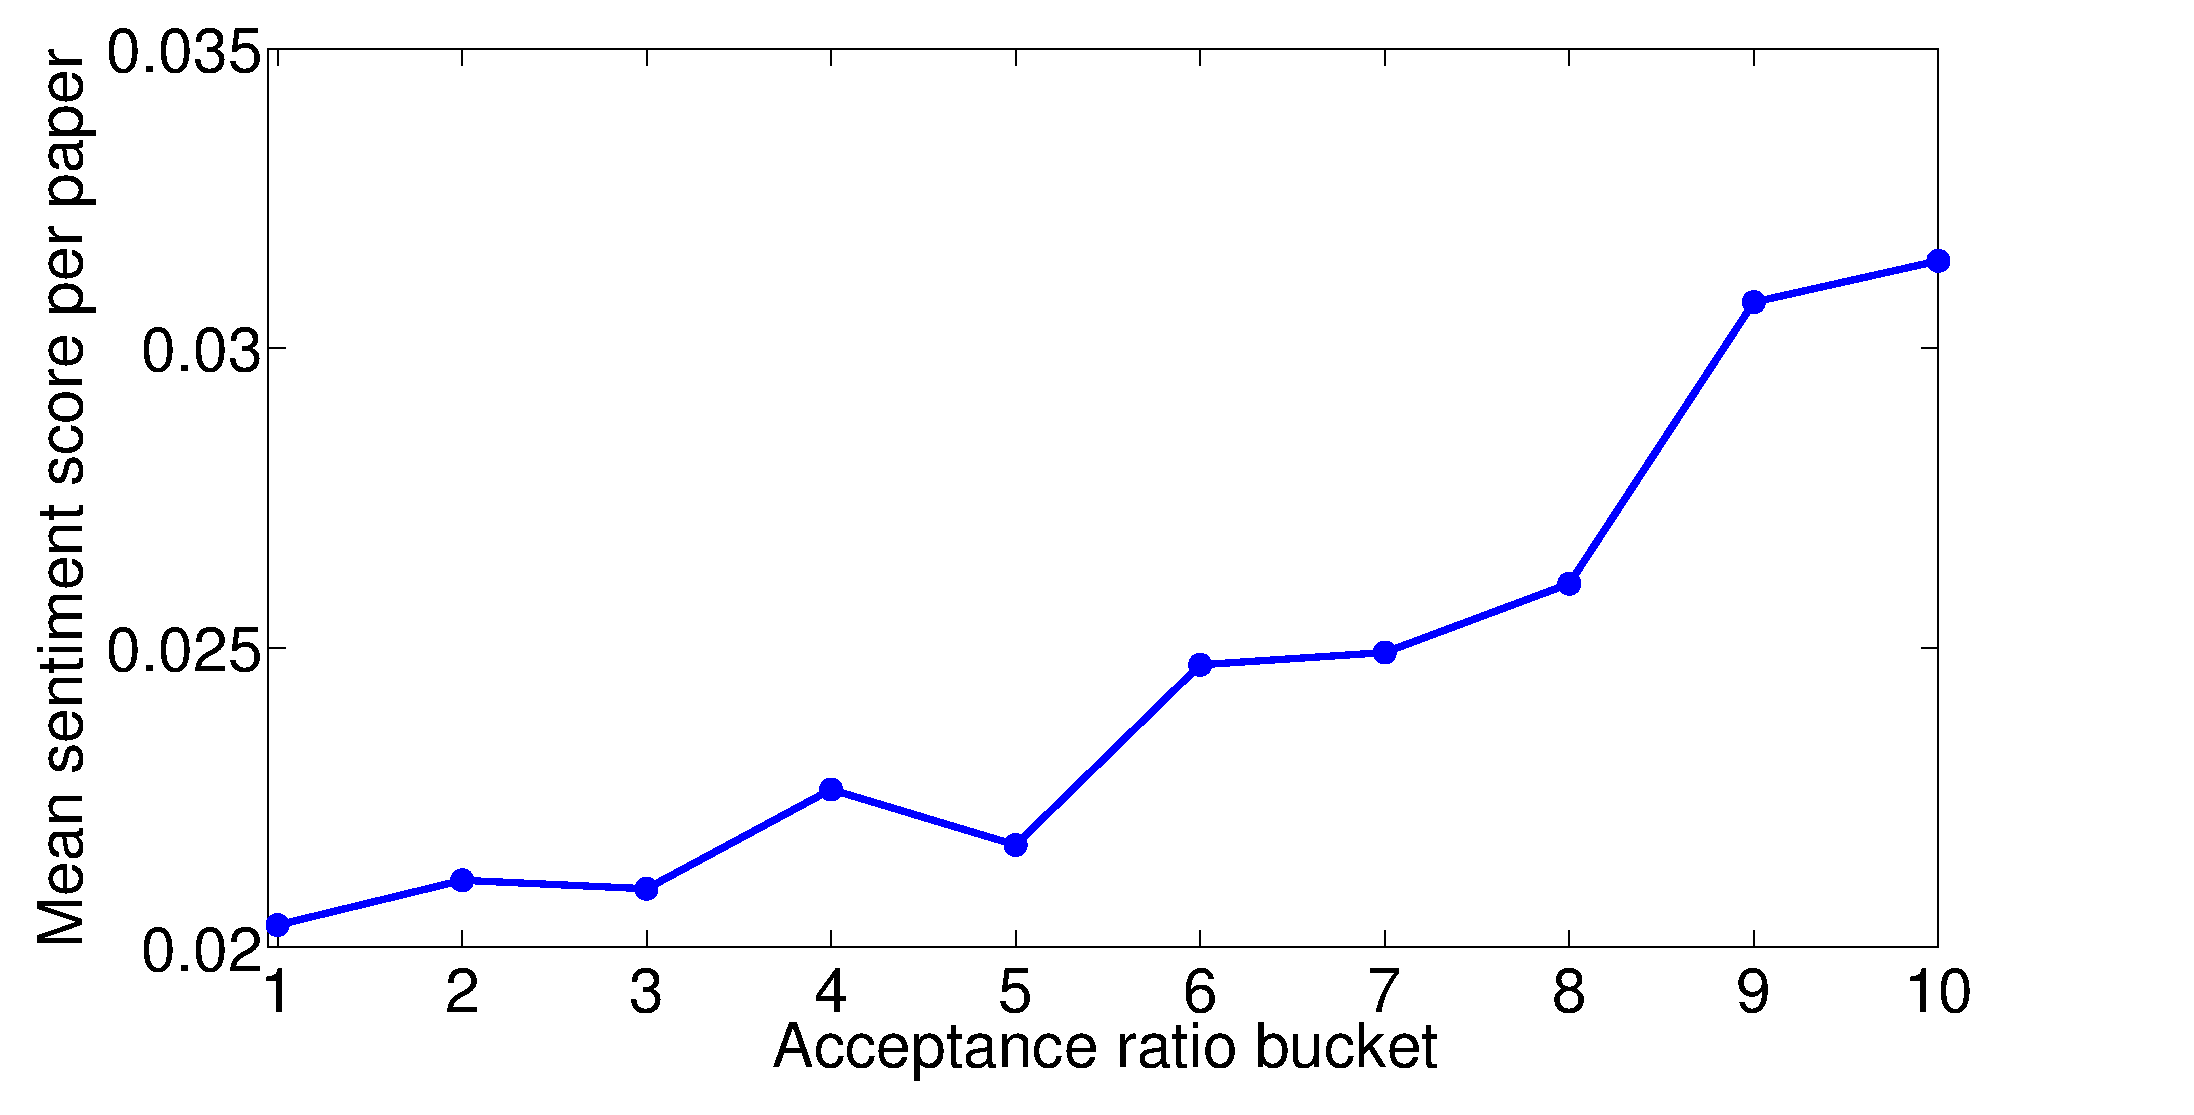
\includegraphics[scale=0.15]{figures/sentiment_succes_ratio-eps-converted-to.pdf}
\end{tabular}
\caption{{\bf (Left)} Mean number of citations per paper versus acceptance ratio. {\bf (Middle)} Mean number of reviews per paper versus acceptance ratio. {\bf (Right)} Mean sentiment score per paper versus acceptance ratio. Note that in each case we use acceptance ratio buckets where buckets correspond to acceptance ratio ($\geq 0.1$ and $< 0.2$), ($\geq 0.2$ and $<0.3$) and so on.}
\label{fig13}
\end{figure*}
\subsubsection{Author reputation (AR)} We analyze whether there are some specific authors whose papers always get accepted and similarly there are others whose papers always get rejected.  
For each author we define a metric called {\bf acceptance ratio} which is the fraction of submitted papers accepted in JHEP. Formally, acceptance ratio of an author $i$ is defined by: $acceptance\,ratio_{i}=\frac{accept_{i}}{accept_{i} + reject_{i}}$.    
where $accept_{i}$ and $reject_{i}$ represents respectively the number of accepted and rejected papers of the author $i$ in JHEP. We use this metric as a proxy for author reputation.
We observe that mean acceptance ratio across all the authors is $0.56$. In fact, for almost 7\% of the authors, the acceptance ratio is 1. Next we check whether the authors with high acceptance ratio have higher citations per paper. To this aim we segregate authors based on the acceptance ratio and calculate the mean number of citations per paper for these authors (refer to fig.~\ref{fig13}{\bf (Left)}). We observe an increasing trend suggesting that the authors with higher acceptance ratio tend to have higher citations. 
\begin{figure}
\centering
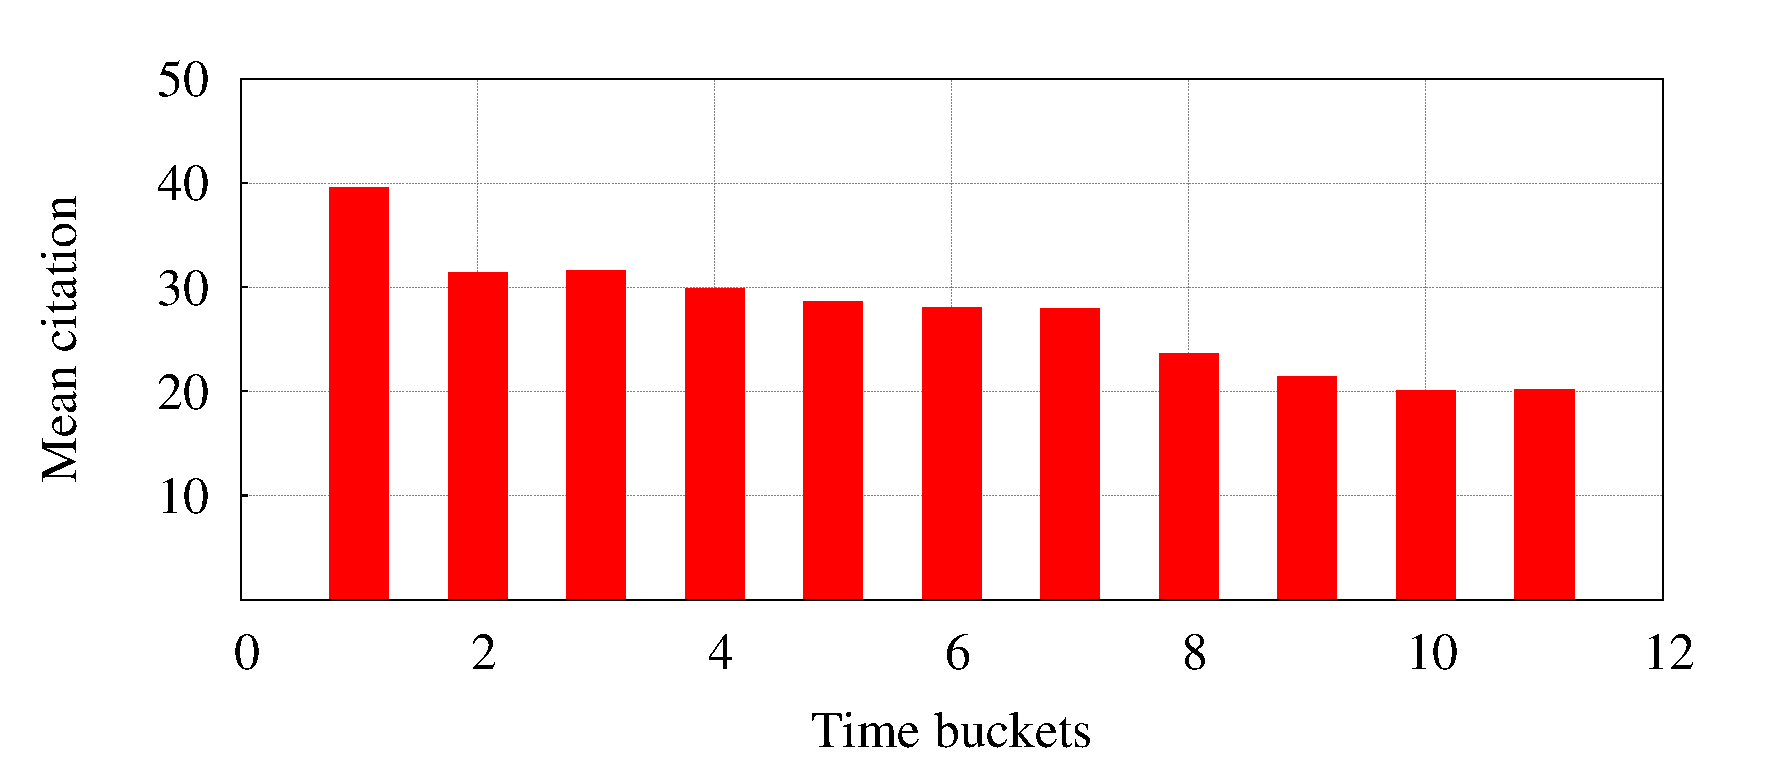
\includegraphics[scale=0.25]{figures/prod_citation.eps}
\caption{Mean citation of the papers versus the average time(in days) between two submission. Note that  we use time buckets where buckets correspond to $<100$,($\geq 100$ and $< 200$), ($\geq 200$ and $<300$) and so on.\vspace{-2mm}}
\label{fig:prod}
\end{figure}

To check whether the authors having higher acceptance ratio are also reviewed less, we again segregate the authors based on the acceptance ratio and calculate the average number of reviews received per paper for these authors (refer to fig.~\ref{fig13}{\bf (Middle)}). We observe a decreasing trend implying that papers of authors with higher acceptance ratio are indeed reviewed less. Although there are authors with high acceptance ratio whose papers are reviewed less, they are often highly cited indicating the overall effectiveness of the review process. We further study the sentiment score of the review reports for authors with different acceptance ratios. For authors in a given  acceptance ratio bucket we calculate the average sentiment score of the review reports of their papers.
We observe that the authors having higher acceptance ratios tend to have more positive reviews on average compared to the others with lower acceptance ratios which is indicated by the increasing trend in the curve in fig.~\ref{fig13}{\bf (Right)}. 

\subsubsection{Author productivity (AP)} It is established in the literature \cite{yan2012better} that the more papers an author publishes, more are his chances of getting cited. We hence use it as a feature in predicting the long-term citation of the paper. We calculate for each author the mean time ($s_t$) between two submissions. We use $s_t$ as proxy for author productivity as low $s_t$ would indicate higher productivity rate and vice versa.  
The papers are segregated based on the corresponding author's $s_t$ and then the mean citation is calculated. Each bucket correspond to $<100$,($\geq 100$ and $< 200$), ($\geq 200$ and $<300$) and so on. We observe that more frequent the submission, more is the chance of getting citation (refer to figure \ref{fig:prod}).


%\medskip